\chapter{Lecture 5}

This lecture is about \texttt{Support Vector Machines and Convex
Optimization} where chapter \texttt{ESL Chapter 4.5, 12.1,
12.2 and 12.3.1} should be looked upon.

\begin{itemize}
  \item Convex optimization using Lagrange multipliers
  \item Optimal Separating Hyperplanes
  \item Support Vector Machines
  \item The Kernel trick
\end{itemize}

\section{Constrained Optimization}

We learn to solve

\begin{align}
  max_x & f(x) \\
  g(x) =  & 0 \\
  h(x) \geq & 0
\end{align}

using Lagrange multipliers

\subsection{Unconstrained optimization}

Assume that $f$ is nice, i.e. continuously differentiable

Then a local maxima, $x*$ fulfills, that gradient is zero $\nabla_x f(x*) = 0$ and the Hessian is negative definite, $v^T \nabla^2_{xx} f(x*) v < 0, \forall v \in \mathbb{R}^n$

where

\[
    \nabla_x f(x) = \left(
    \begin{array}{c}
      \frac{\partial f(x)}{\partial x_1} \\
      \vdots \\
      \frac{\partial f(x)}{\partial x_n}
    \end{array}\right)
\]

and

\[
    \nabla_{xx}^2 f(x) = \left(
    \begin{array}{ccc}
      \frac{\partial^2 f(x)}{\partial x^2_1} & \cdots & \frac{\partial^2 f(x)}{\partial x_1 \partial x_n} \\
      \vdots & \ddots & \vdots \\
      \frac{\partial^2 f(x)}{\partial x^n \partial x_1} & \cdots & \frac{\partial^2 f(x)}{\partial x^2_n}
    \end{array} \right)
\]

A negative second derivative guarantees a local maximum (otherwise a saddle point or local minimum).

\subsection{Constrained optimization}

We introduce a constraint that $x$ must fulfill $max_x f(x)$ with $g(x) = 0$. The stationary points are defined by $\nabla f = -\lambda \nabla g$ for some constant $\lambda$

We define the Lagrange primal function

\[
    L(x, \lambda) = f(x) + \lambda g(x)
\]

and the Lagrange multiplier $\lambda$

We wish to find a solution $(x*, \lambda*)$ to $\max\limits_x \min\limits_x L(x, \lambda)$ by solving

\[
    \frac{\partial L}{\partial x} = 0
\]

and

\[
    \frac{\partial L}{\partial \lambda} = 0
\]

which is the same as $\nabla L(x, \lambda) = 0$

The stationary points, $x*$, might be local maxima, local minima or saddle points. Verify that the Hessian is negative semi-definite.

One example from lecture \cite[p.~8]{lecture5}, where we $\max_x f(x_1, x_2) = 1 - x_1^2 - x_2^2$ with constraint $g(x_1, x_2) = x_1 + x_2 -1 = 0$

The Lagrangian is

\[
    L(\bm{x}, \lambda) = f(x) + \lambda g(x) = 1 - x_1^2 - x_2^2 + \lambda (x_1 + x_2 -1)
\]

were we $\nabla L(\bm{x}, \lambda) = 0$ and then we have 3 functions with 3 unknown and the solution is $(x_1^*, x_2^*, \lambda) = (1/2, 1/2, 1)$

\subsection{Inequality constraints}

Constrained optimization with inequality constraints with $max_x f(x)$ with $h(x) \geq 0$.

The optimum is either within the feasible region $h(x) \geq 0$ or along the edge $h(x) = 0$, see the lecture \cite[p.~9]{lecture5} for pictures

Notice that $\nabla h$ is always pointing inwards since $h > 0$ in the feasible region and $h=0$ along the edge.


The Lagranges problem for inequality constraints, a local maximum to the constrained optimization problem with $max_x f(x)$ with $h(x) \geq 0$ then the Lagrange function is

\[
    L(x, \mu) = f(x) = \mu h(x)
\]

is given by $(x*, \mu *) $ when KKT conditions are

\begin{itemize}
  \item $\nabla_x L(x*, \mu *) = 0$
  \item $\mu* \geq 0$
  \item $\mu * h(x*) = 0$ complementarity conditions
  \item $h(x*) \geq 0$
  \item Negative definite constraints on Hessian
\end{itemize}

For a minimization problem we change sigh $L(x, \mu) = f(x) - \mu h(x)$

\subsection{Multiple constraints}

Constrained optimization with inequality constraints and equality with $max_x f(x)$ with $h(x) \geq 0$ and $g(x) = 0$ then the Lagrange multipliers $L(x , \lambda, \mu) = f(x) + \sum_{j} \lambda_j g_j (x) + \sum_{k} \mu_k h_k (x)$

\subsection{Lagrange dual problem}

The Lagrange primal problem is

\[
    \max\limits_x \min\limits_\lambda L(x, \lambda, \mu)
\]

If we swap the order of min and max we get the Lagrange dual
problem,

\[
    \min\limits_\lambda \max\limits_x L(x, \lambda, \mu)
\]

Often these two problems have the same solution, where we define Lagrange dual function

\[
    L_D(\lambda, \mu) = \max\limits_x L_p (x, \lambda, \mu)
\]

From lecture \cite[p.~14]{lecture5} then Slater's condition says

\begin{quote}
  The primal and dual optimization problems are equivalent when $f$ is concave and constraints are convex.
\end{quote}

\begin{itemize}
  \item There must be some $x$ fulfilling all constraints
  \item Linear constraints are OK
  \item A local optimum will also be the global optimum
  \item Not necessary to check conditions on the Hessian
\end{itemize}

\section{Optimal Separating Hyperplane}

From the lecture slides \cite[p.~16]{lecture5} then

\begin{itemize}
  \item Binary classification
  \item Sometimes data are perfectly separated by a straight line
  \item No overlap, one class on one side and the other class on the other side
  \item Not very useful in practice but it can be modified into the powerful Support Vector Machine
\end{itemize}

From the book \cite[p.~130]{friedman2016elements}

We have seen that linear discriminant analysis and logistic regression both estimate linear decision boundaries in similar but slightly different ways.

These procedures construct linear decision boundaries that explicitly try to separate the data into different classes as well as possible. They provide the basis for support vector classifiers.

With a linear decision functions $y_\text{new}  = \text{sign}(x_\text{new} \beta + \beta_0) $

For practical reason we label the two classes $1$ and $-1$, where fitting the model involves choosing values for $\beta$ and $\beta_0$.

Binary classification, extensions can be made as "One vs. the rest" and "One vs one" both approaches uses several models.

So we need a \textbf{decision function}, Many hyperplanes can separate the two classes, what would be the optimal?

\section{Support Vector Machine}

From lecture \cite[p.~31]{lecture5} we have the SVM. Most classification problems have overlapping classes, where we modify the (Optimal separating hyperplanes) OSH such that we allow for some overlap. This is where SVM comes in, where we use this together with the kernel trick SVM is on of our most flexible classifiers.

From OSH we got

\[
    \arg \min\limits_{\beta, \beta_0} \frac{1}{2} ||\beta ||^2
\]
such that
\[
    y_i (x_i \beta - \beta_0) \geq 1 \quad \forall i
\]

Now we do allow some overlap

\[
    \arg \min\limits_{\beta, \beta_0} \frac{1}{2} ||\beta ||^2 + \lambda \sum_{i=1}^{n} \xi_i
\]

such that

\begin{equation}
    \begin{split}
       y_i (x_i \beta - \beta_0) & \geq 1 - \xi_i \quad \forall i \\
        \xi_i & \geq 0 \quad \forall i
    \end{split}
\end{equation}

We give our self a budget for overlap. Smaller budget - larger $\lambda$ - noisier solution

\begin{figure}[H]
  \centering
  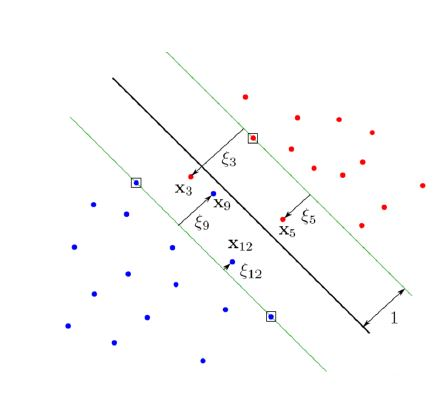
\includegraphics[width=0.9\textwidth]{SVMexample}
\end{figure}

So our SVM is defined as

\[
    \arg \min\limits_{\alpha} \alpha \bm{1} - \frac{1}{2} \alpha^T Y XX^T Y \alpha
\]

such that

\begin{equation}
    \begin{split}
       0 \leq \alpha_i \leq \lambda & \forall i \\
       \sum \alpha_i y_i & = 0
    \end{split}
\end{equation}
Both are quadratic programming problems with linear constraints. More can be seen on lecture \cite[p.~34-35]{lecture5}



\section{Basis expansion and kernels}


\begin{itemize}
  \item We can do SVM (and OSH) on a transformed feature space
  \item Transformed features gives non-linear decision boundaries.
  \item With the Kernel trick we can use an infinite dimensional feature expansion
\end{itemize}

We use $h(X)$ instead of $X$

\[
    \arg \min\limits_{\alpha} \alpha \bm{1} - \frac{1}{2} \alpha^T Y h(X)h(X)^T Y \alpha
\]

such that

\begin{equation}
    \begin{split}
       0 \leq \alpha_i \leq \lambda & \forall i \\
       \sum \alpha_i y_i & = 0
    \end{split}
\end{equation}

So the term $h(X)h(X)^T$ does not depend on $M$, the number of basis functions.

We only need to specify $K(X)$ such that $h(X)h(X)^T = K(X)$ we call $K$ a kernel. Then $h$ is implicitly defined by $K$. 

The common kernels can be seen on lecture \cite[p.~38]{lecture5}

\[
    \arg \min\limits_{\alpha} \alpha \bm{1} - \frac{1}{2} \alpha^T Y K(X)Y \alpha
\]

such that

\begin{equation}
    \begin{split}
       0 \leq \alpha_i \leq \lambda & \forall i \\
       \sum \alpha_i y_i & = 0
    \end{split}
\end{equation}

So to classify a new observation

\[
    \begin{split}
       \hat{y}_\text{new}  & = sign(\beta h(x_\text{new} + \beta_0) \\
         & = sign \left( \sum_{i=1}^{n} \alpha_i y_i K(x_\text{new}, x_i) + b_0 \right)
    \end{split}
\]

calculate $b_0$ using one of the points, $i$, on the margin

\[
    b_0 = y_i - \sum_{j=1}^{n} \alpha_j y_j K(x_i, x_j)
\]

We have found an efficient way of maximizing the margin
between classes and select parameters using cross validation. \cite[p.~40,43]{lecture5}

Problem is, that Kernel methods do not scale well. Limited to around 10000-20000 observations. Kernel methods do not do variable selection in any reasonable or
automatic way, e.g. With more features than observations there is always a separating hyperplane.\\

Other problem is, Potential problem with large number of features if many of them are garbage







Furthermore look at lecture \cite[p.~3-6]{lecture6}